\documentclass[10pt,a5paper]{article}
\usepackage[margin=1cm]{geometry}
\usepackage[utf8]{inputenc}
\usepackage[IL2]{fontenc}
\usepackage[czech]{babel}
\usepackage{microtype}
\usepackage{amssymb}
\usepackage{amsthm}
\usepackage{amsmath}
\usepackage{xcolor}
\usepackage{graphicx}
\usepackage{wasysym}
\usepackage{multicol}

\usepackage[inline]{enumitem}

\newcommand{\R}{\mathbb{R}}

\newcommand{\hint}[1]{{\color{gray}\footnotesize\noindent(Nápověda: #1)}}

\setlist[enumerate]{label={(\alph*)},topsep=\smallskipamount,itemsep=1.25\bigskipamount,parsep=0pt}
\setlist[itemize]{topsep=\smallskipamount,noitemsep}

\def\tisk{%
\newbox\shipouthackbox
\pdfpagewidth=2\pdfpagewidth
\let\oldshipout=\shipout
\def\shipout{\afterassignment\zdvojtmp \setbox\shipouthackbox=}%
\def\zdvojtmp{\aftergroup\zdvoj}%
\def\zdvoj{%
    \oldshipout\vbox{\hbox{%
        \copy\shipouthackbox
        \hskip\dimexpr .5\pdfpagewidth-\wd\shipouthackbox\relax
        \box\shipouthackbox
    }}%
}}%



\newtheorem*{poz}{Pozorování}

\theoremstyle{definition}
\newtheorem{uloha}{\atr Úloha}
\newtheorem{suloha}[uloha]{\llap{$\star$ }Úloha}
\newtheorem*{bonus}{Bonus}
\newtheorem*{defn}{Definice}

\pagestyle{empty}

\let\ee\expandafter

\def\vysld{}
\let\printvysl\relax
\let\printalphvysl\relax

\makeatletter
\long\def\vysl#1{\ee\ee\ee\gdef\ee\ee\ee\vysld\ee\ee\ee{\ee\vysld\ee\printvysl\ee{\the\c@uloha}{#1}}}
\let\vyslplain\vysl

\def\locvysl#1{\ee\gdef\ee\locvysld\ee{\locvysld\item #1}}
\let\lv\locvysl

\newenvironment{ulohav}[1][]{\begin{uloha}[#1]\gdef\locvysld{\begin{enumerate}}}{\ee\vyslplain\ee{\locvysld\end{enumerate}}\end{uloha}}
%

\def\stitem{\@noitemargtrue\@item[$\star$ \@itemlabel]}

\makeatother

\def\atr{}
\def\basic{\def\atr{\llap{\mdseries$\sun$ }\gdef\atr{}}}
\def\interest{\def\atr{\llap{$\star$ }\gdef\atr{}}}
\let\mb\mathbf

\let\la\langle
\let\ra\rangle
\def\bla{\bigl\la}
\def\bra{\bigr\ra}
\def\blz{\bigl(}
\def\brz{\bigr)}

\def\R{\mathbb{R}}
\def\N{\mathbb{N}}

\begin{document}

% \tisk


\section*{Procvičování kvadratických nerovnic atd.}

\begin{uloha}
% tato úloha je do značné míry řešitelná i jen podíváním se na absolutní člen...
Který graf je grafem které kvadratické funkce?

\hbox to\hsize{%
\vbox{\hsize=.3\hsize \linewidth=.3\linewidth
\begin{enumerate}[label={(\arabic*)}]
    \item $x^2-6 x+9$
    \item $x^2-2 x$
    \item $2 x^2-2 x-12$
    \item $x^2-1$
    \item $-x^2-2 x-1$
    \item $-x^2-5 x-6$
\end{enumerate}
}\hfil
\hbox{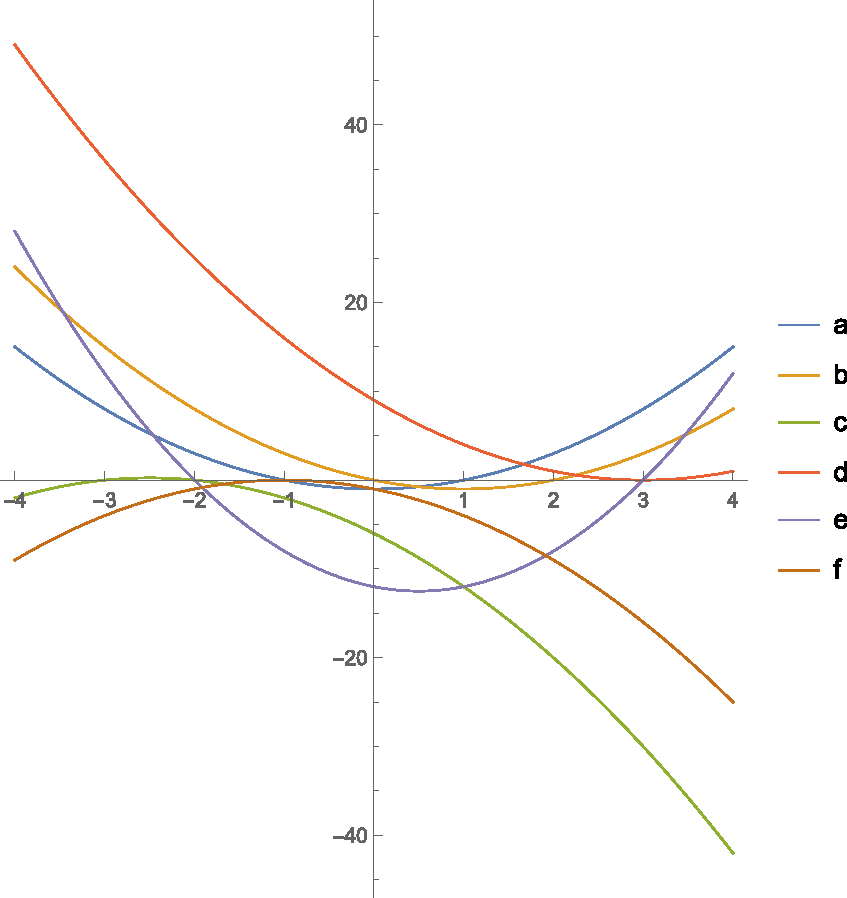
\includegraphics[width=.7\hsize]{paraboly_legend.pdf}}%
}
\vysl{1d, 2b, 3e, 4a, 5f, 6c}
\end{uloha}



\begin{ulohav}
\everymath{\displaystyle}
Vyřešte nerovnice:
\begin{multicols}{2}
\begin{enumerate}
    \item $(x+44)(x-55) \leq 0$\lv{$\la-44;55\ra$}
    \item $x^2-11 x-2420 \leq 0$\lv{$\la-44;55\ra$}
    \item $x^2 > \pi$\lv{$\blz-\infty;-\sqrt{\pi}\brz\cup \blz\sqrt\pi; \infty\brz$}
    \item $x^2 > -777$\lv{$\R$}
    \item $x^2 + 2x \leq -1$\lv{$\{-1\}$}
    \item $3x - 2x^2 > 2$\lv{$\emptyset$}
    \item $(x + 1) (x + 2) < (x + 3) (x + 4)$\lv{$\blz-\frac52;\infty\brz$}
    \item $(x + 1) (x + 2) < (2x + 3) (x + 4)$\lv{$\blz-\infty; -4-\sqrt6\brz \cup \blz-4+\sqrt6; \infty\brz$}
    \item $(x^2 + 4 x - 2) (x + 3) < 0$\lv{$\blz-\infty; -2-\sqrt6\brz \cup \blz-3; -2+\sqrt6\blz$}
    \item $(x^2 + 4 x - 2) (x^2 + 4 x + 2) > 0$\lv{$\blz-\infty;-2-\sqrt6\brz \cup \blz -2-\sqrt2; -2+\sqrt2 \brz \cup \blz-2+\sqrt6; \infty\brz$}
    \item $\frac{x^2 + 4 x - 2}{x^2 + 4 x + 2} \geq 0$\lv{$\blz-\infty;-2-\sqrt6\bra \cup \blz -2-\sqrt2; -2+\sqrt2 \brz \cup \bla-2+\sqrt6; \infty\brz$}
    \item $x^3+2 x^2+x+2 \geq 0$\lv{$\langle-2;\infty)$}
\end{enumerate}
\end{multicols}
\end{ulohav}

\interest
\begin{uloha}
Pro které hodnoty čísla $c \in \R$ má kvadratická nerovnice $2 x^2 + 7 x + c \geq 0$ množinu řešení $\R$?\vysl{$c \in \bla\frac{49}{8}, \infty\brz$}
\end{uloha}


\newpage
\parindent=0pt
\parskip=\smallskipamount
\def\printvysl#1#2{\textbf{#1.}\ #2\par}
\vysld


\end{document}

